%%%%%%%%%%%%%%%%%%%%%%%%%%%%%%%%%%%%%%%%%%%%%%%%%%%%%%%%%%%%%%%%%%%%%%%%%%%%%%%
% CASE STUDY TEMPLATE - Programming and Problem Solving
% Author: Brendan Shea, PhD
% Course: Programming and Problem Solving
% Rochester Community and Technical College
%%%%%%%%%%%%%%%%%%%%%%%%%%%%%%%%%%%%%%%%%%%%%%%%%%%%%%%%%%%%%%%%%%%%%%%%%%%%%%%

\documentclass[11pt,letterpaper]{article}

%---------- PACKAGES ----------%
\usepackage[margin=1in, headheight=22pt]{geometry}
\usepackage[T1]{fontenc}
\usepackage{xcolor}
\usepackage{tcolorbox}
\usepackage{graphicx}
\usepackage{titlesec}
\usepackage{enumitem}
\usepackage{fancyhdr}
\usepackage{listings}
\usepackage{hyperref}
\usepackage{multicol}
\usepackage{booktabs}
\usepackage{tikz}
\usepackage{float}
\usepackage{amssymb}
\usepackage{amsmath}
\usepackage{pifont}

% TikZ libraries
\usetikzlibrary{shapes.geometric, arrows.meta, positioning, calc,
                backgrounds, fit, matrix, decorations.pathreplacing, chains}

% Load tcolorbox libraries
\tcbuselibrary{skins,breakable,listings,listingsutf8}

%---------- COLOR DEFINITIONS ----------%
\definecolor{csprimary}{HTML}{2C3E50}
\definecolor{cssecondary}{HTML}{E74C3C}
\definecolor{cstertiary}{HTML}{3498DB}
\definecolor{csaccent}{HTML}{27AE60}
\definecolor{cswarm}{HTML}{F39C12}
\definecolor{cslight}{HTML}{ECF0F1}
\definecolor{csdark}{HTML}{1A252F}

% Syntax highlighting colors
\definecolor{codegreen}{HTML}{27AE60}
\definecolor{codepurple}{HTML}{9B59B6}
\definecolor{codeorange}{HTML}{E67E22}
\definecolor{codeblue}{HTML}{3498DB}
\definecolor{codegray}{HTML}{95A5A6}
\definecolor{codestring}{HTML}{E74C3C}
\definecolor{codebg}{HTML}{1E2A38}

%---------- CASE STUDY METADATA ----------%
\newcommand{\cstitle}{Code as a Microscope}
\newcommand{\cssubtitle}{How Computational Models Drive Scientific Discovery}
\newcommand{\csauthor}{Brendan Shea, PhD}
\newcommand{\cscourse}{Programming and Problem Solving}
\newcommand{\csinstitution}{Rochester Community and Technical College}
\newcommand{\csdate}{\today}

%---------- LISTINGS CONFIGURATION ----------%
\lstdefinestyle{basestyle}{
    backgroundcolor=\color{codebg},
    basicstyle=\ttfamily\small\color{white},
    breakatwhitespace=false,
    breaklines=true,
    captionpos=b,
    keepspaces=true,
    showspaces=false,
    showstringspaces=false,
    showtabs=false,
    tabsize=4,
    frame=none,
    xleftmargin=4mm,
    xrightmargin=4mm,
    aboveskip=0pt,
    belowskip=0pt,
}

\lstdefinestyle{javastyle}{
    style=basestyle,
    language=Java,
    keywordstyle=\color{codeblue}\bfseries,
    commentstyle=\color{codegray}\itshape,
    stringstyle=\color{codestring},
    morekeywords={String, Scanner, System, var, boolean, Math, List, Map,
                  HashMap, ArrayList, Random, record},
}

%---------- CUSTOM ENVIRONMENTS ----------%
\newcommand{\keyterm}[1]{\textbf{\textcolor{cssecondary}{#1}}}

\newtcolorbox{conceptbox}[1][]{
    enhanced,
    colback=cslight,
    colframe=csprimary,
    fonttitle=\bfseries\color{white},
    title=#1,
    attach boxed title to top left={yshift=-2mm, xshift=5mm},
    boxed title style={colback=csprimary},
    breakable
}

\newtcolorbox{historybox}[1][]{
    enhanced,
    colback=codepurple!8,
    colframe=codepurple,
    fonttitle=\bfseries\color{white},
    title=#1,
    attach boxed title to top left={yshift=-2mm, xshift=5mm},
    boxed title style={colback=codepurple},
    breakable
}

\newtcolorbox{tipbox}[1][]{
    enhanced,
    colback=csaccent!8,
    colframe=csaccent,
    fonttitle=\bfseries\color{white},
    title=#1,
    attach boxed title to top left={yshift=-2mm, xshift=5mm},
    boxed title style={colback=csaccent},
    breakable
}

\newtcolorbox{warningbox}[1][]{
    enhanced,
    colback=cssecondary!8,
    colframe=cssecondary,
    fonttitle=\bfseries\color{white},
    title=#1,
    attach boxed title to top left={yshift=-2mm, xshift=5mm},
    boxed title style={colback=cssecondary},
    breakable
}

\newtcolorbox{debatebox}[1][]{
    enhanced,
    colback=cswarm!8,
    colframe=cswarm,
    fonttitle=\bfseries\color{white},
    title=#1,
    attach boxed title to top left={yshift=-2mm, xshift=5mm},
    boxed title style={colback=cswarm},
    breakable
}

\newtcolorbox{quotebox}[1][]{
    enhanced,
    colback=cstertiary!8,
    colframe=cstertiary,
    fonttitle=\bfseries\color{white},
    title=#1,
    attach boxed title to top left={yshift=-2mm, xshift=5mm},
    boxed title style={colback=cstertiary},
    breakable
}

\newtcblisting{javacode}[1][]{
    enhanced,
    colback=codebg,
    colframe=csaccent,
    colupper=white,
    fonttitle=\bfseries\color{white},
    title=#1,
    attach boxed title to top left={yshift=-2mm, xshift=5mm},
    boxed title style={colback=csaccent},
    left=0mm, right=0mm, top=2mm, bottom=2mm,
    boxrule=1pt,
    breakable,
    pad at break=2mm,
    listing only,
    listing options={style=javastyle}
}

\newtcolorbox{questionbox}{
    enhanced,
    colback=cswarm!10,
    colframe=cswarm,
    fonttitle=\bfseries\color{white},
    title=Discussion Questions,
    attach boxed title to top center={yshift=-2mm},
    boxed title style={colback=cswarm},
    breakable
}

\newtcolorbox{glossarybox}{
    enhanced,
    colback=cslight,
    colframe=csprimary,
    fonttitle=\bfseries\color{white},
    title=Glossary of Key Terms,
    attach boxed title to top center={yshift=-2mm},
    boxed title style={colback=csprimary},
    breakable
}

%---------- HEADER/FOOTER ----------%
\pagestyle{fancy}
\fancyhf{}
\fancyhead[L]{\small\textcolor{csprimary}{\cscourse}}
\fancyhead[R]{\small\textcolor{csprimary}{Case Study}}
\fancyfoot[C]{\thepage}
\renewcommand{\headrulewidth}{0.4pt}
\renewcommand{\headrule}{\hbox to\headwidth{\color{csprimary}\leaders\hrule height \headrulewidth\hfill}}

%---------- SECTION FORMATTING ----------%
\titleformat{\section}
    {\Large\bfseries\color{csprimary}}
    {\thesection}{1em}{}[\color{cssecondary}\titlerule]

\titleformat{\subsection}
    {\large\bfseries\color{cstertiary}}
    {\thesubsection}{1em}{}

%---------- HYPERLINK SETTINGS ----------%
\hypersetup{
    colorlinks=true,
    linkcolor=cstertiary,
    urlcolor=cstertiary
}

%%%%%%%%%%%%%%%%%%%%%%%%%%%%%%%%%%%%%%%%%%%%%%%%%%%%%%%%%%%%%%%%%%%%%%%%%%%%%%%
\begin{document}

%---------- TITLE BLOCK ----------%
\begin{tcolorbox}[
    enhanced,
    colback=csprimary,
    colframe=csprimary,
    arc=0mm,
    left=10mm, right=10mm, top=8mm, bottom=8mm
]
\begin{center}
    {\huge\bfseries\color{white}\cstitle}\\[3mm]
    {\Large\color{cslight}\cssubtitle}\\[5mm]
    \textcolor{cssecondary}{\rule{0.5\textwidth}{1pt}}\\[5mm]
    {\large\color{white}\csauthor}\\[2mm]
    {\normalsize\color{cslight}\cscourse\ $\bullet$ \csinstitution}
\end{center}
\end{tcolorbox}

\vspace{5mm}

%---------- INTRODUCTION ----------%
\section*{Introduction}

In 1687, Isaac Newton published equations describing gravity and motion. In 1846, astronomers used those equations---purely by hand calculation---to predict the existence and location of an undiscovered planet. When they pointed their telescope to the predicted spot, Neptune was there. Mathematics had reached beyond what any telescope could see.

Computing extended this power by orders of magnitude. Today, researchers simulate the collision of galaxies, track the spread of pandemics across billions of people, fold proteins that biology hasn't yet synthesized, and forecast the global climate decades into the future. These are not experiments in the traditional sense---no lab bench, no test tube. They are \keyterm{computational models}: carefully constructed programs that capture the rules of a system and let us watch what happens when we run them.

This case study is about that idea. What is a model? How do you turn one into code? What have scientists discovered because of computers that they could never have discovered without them? And what are the limits---the ways that models can mislead as well as illuminate?

\begin{conceptbox}[The Three Pillars of Modern Science]
Scientists traditionally acquire knowledge in two ways:

\textbf{Theory:} Deriving consequences from mathematical principles. Newton's laws, quantum mechanics, evolution by natural selection---theoretical frameworks that explain and predict.

\textbf{Experiment:} Testing hypotheses in controlled conditions. Measuring what nature actually does when you intervene.

Since the mid-twentieth century, a third pillar has emerged:

\textbf{Computation:} Simulating systems too complex for closed-form mathematics and too large (or dangerous, or slow, or expensive) for direct experiment. Climate systems, protein structures, population dynamics, galaxy formation---science that lives in the computer.

Many scientists today work primarily at this third pillar. Their laboratory is a cluster of servers; their instruments are programs.
\end{conceptbox}

%---------- WHAT IS A MODEL ----------%
\section{What Is a Model?}

\subsection{Simplification by Design}

The word ``model'' is used in many ways---a model airplane, a fashion model, a role model. In science and engineering, a \keyterm{model} has a specific meaning: a simplified representation of a system, designed to capture the features that matter for a particular question while ignoring those that don't.

That last part is crucial. A model is \textit{not} a perfect replica of reality. It is a deliberate simplification. The statistician George Box captured this in a famous aphorism:

\begin{quotebox}[George Box (1976)]
``All models are wrong, but some are useful.''
\end{quotebox}

A weather forecast model doesn't track every air molecule---there are $10^{44}$ of them. It divides the atmosphere into grid cells, perhaps 10 kilometers on a side, and tracks average conditions in each cell. This is ``wrong'' in the sense that it misses sub-grid phenomena. It is ``useful'' in the sense that it correctly predicts tomorrow's rain.

The art of modeling is knowing what to include and what to leave out. Include too little and the model misses the phenomena you care about. Include too much and the model becomes as complicated as reality itself---impossible to understand, expensive to run, and no more useful than nature.

\subsection{Types of Models}

Scientific models take many forms, but a few categories appear repeatedly:

\begin{center}
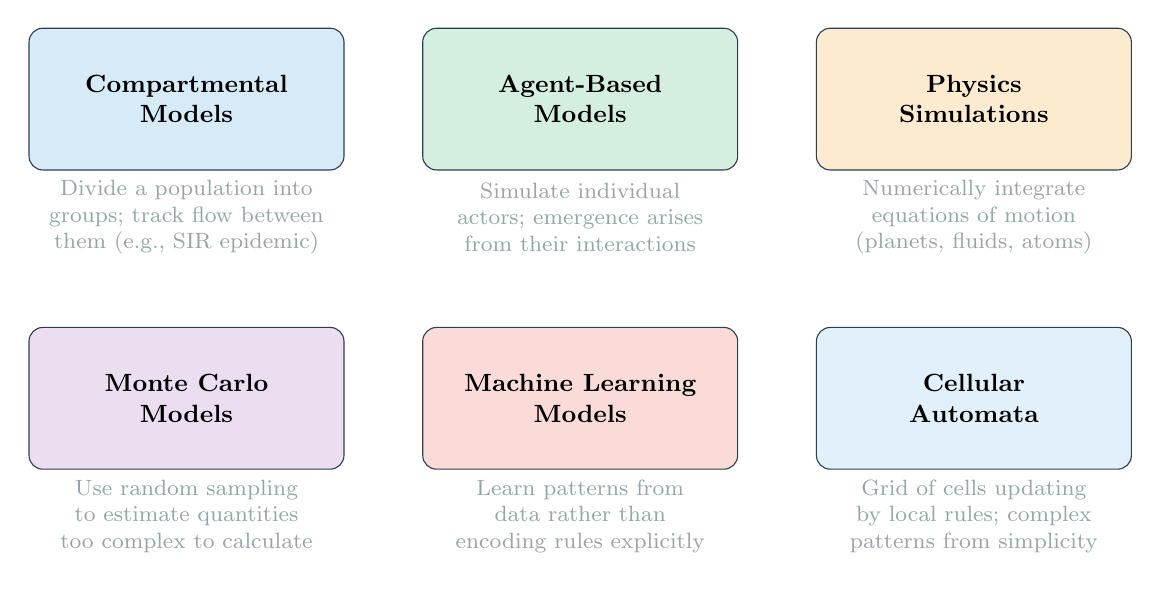
\begin{tikzpicture}[
    mtype/.style={rectangle, rounded corners=5pt, draw=csprimary, fill=#1,
                  minimum width=40mm, minimum height=18mm, align=center, font=\small\bfseries},
    desc/.style={font=\footnotesize, color=codegray, align=center, text width=38mm}
]
\node[mtype=cstertiary!20]  (comp)  at (0,0)    {Compartmental\\ Models};
\node[desc] at (0,-1.5)  {Divide a population into\\groups; track flow between\\them (e.g., SIR epidemic)};

\node[mtype=csaccent!20]    (abm)   at (5,0)    {Agent-Based\\ Models};
\node[desc] at (5,-1.5)  {Simulate individual\\actors; emergence arises\\from their interactions};

\node[mtype=cswarm!20]      (phys)  at (10,0)   {Physics\\ Simulations};
\node[desc] at (10,-1.5) {Numerically integrate\\equations of motion\\(planets, fluids, atoms)};

\node[mtype=codepurple!20]  (mc)    at (0,-3.8) {Monte Carlo\\ Models};
\node[desc] at (0,-5.3)  {Use random sampling\\to estimate quantities\\too complex to calculate};

\node[mtype=cssecondary!20] (ml)    at (5,-3.8) {Machine Learning\\ Models};
\node[desc] at (5,-5.3)  {Learn patterns from\\data rather than\\encoding rules explicitly};

\node[mtype=cstertiary!15]  (ca)    at (10,-3.8){Cellular\\ Automata};
\node[desc] at (10,-5.3) {Grid of cells updating\\by local rules; complex\\patterns from simplicity};
\end{tikzpicture}
\end{center}

\subsection{The Modeling Cycle}

Building a useful model is not a one-shot task---it's an iterative process. Scientists cycle through a series of steps, refining their model each time.

\begin{center}
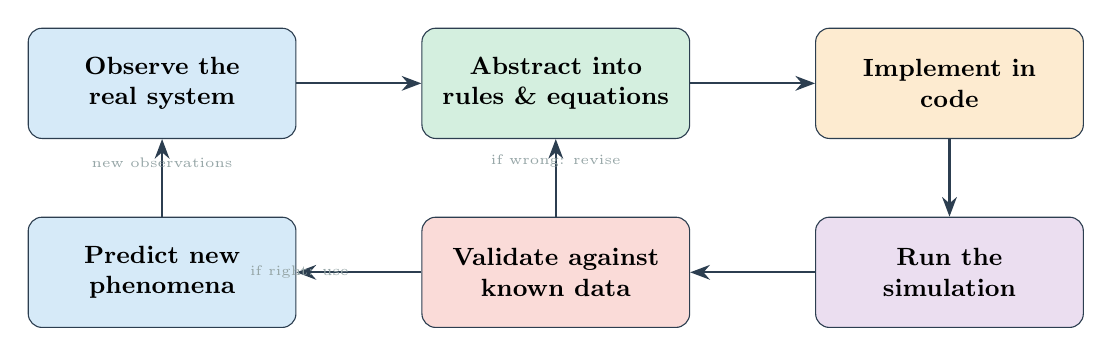
\begin{tikzpicture}[
    step/.style={rectangle, rounded corners=5pt, draw=csprimary, fill=#1,
                 minimum width=34mm, minimum height=14mm, align=center, font=\small\bfseries},
    arrow/.style={-{Stealth[length=2.5mm]}, thick, color=csprimary}
]
\node[step=cstertiary!20] (obs)     at (0,0)    {Observe the\\real system};
\node[step=csaccent!20]   (abstract) at (5,0)   {Abstract into\\rules \& equations};
\node[step=cswarm!20]     (impl)    at (10,0)   {Implement in\\code};
\node[step=codepurple!20] (run)     at (10,-2.4){Run the\\simulation};
\node[step=cssecondary!20](validate) at (5,-2.4){Validate against\\known data};
\node[step=cstertiary!20] (predict) at (0,-2.4) {Predict new\\phenomena};

\draw[arrow] (obs)      -- (abstract);
\draw[arrow] (abstract) -- (impl);
\draw[arrow] (impl)     -- (run);
\draw[arrow] (run)      -- (validate);
\draw[arrow] (validate) -- node[font=\tiny, above, color=codegray] {if wrong: revise} (abstract);
\draw[arrow] (validate) -- node[font=\tiny, left,  color=codegray] {if right: use}    (predict);
\draw[arrow] (predict)  -- node[font=\tiny, above, color=codegray] {new observations} (obs);
\end{tikzpicture}
\end{center}

The \keyterm{validation} step---comparing model output to real-world data---is what separates a scientific model from a guess. A model that has been validated against past observations earns some trust for future predictions. A model that has never been tested against reality is speculation.

%---------- A BRIEF HISTORY ----------%
\section{A Brief History: When Computers Met Science}

\begin{historybox}[ENIAC and the First Scientific Computation (1945)]
The ENIAC (Electronic Numerical Integrator and Computer), completed in 1945, was built to calculate artillery firing tables for the US Army---predicting where a shell would land given angle, charge, and wind. It was immediately repurposed for science. Physicists at Los Alamos used it to model thermonuclear reactions; meteorologists used it to run the first computerized weather forecast (1950).

That first weather forecast took 24 hours of computation to predict 24 hours of weather---not very useful in practice, but a proof of concept for what would become the most consequential application of computing in science.
\end{historybox}

\begin{historybox}[Lorenz and the Discovery of Chaos (1961)]
Edward Lorenz was a meteorologist at MIT running a simple weather simulation on an early computer. One day in 1961, he re-ran a simulation by entering a number from a printout: 0.506 instead of the full stored value of 0.506127. He expected a nearly identical result.

Instead, the simulation diverged wildly. A tiny difference in initial conditions---less than one part in a thousand---produced a completely different weather pattern within a few simulated months.

Lorenz had accidentally discovered \keyterm{chaos theory}: that some systems are exquisitely sensitive to initial conditions, making long-range prediction fundamentally impossible, not just technically difficult. This became known popularly as the \textbf{butterfly effect}---the idea that a butterfly flapping its wings in Brazil could (in principle) set off a tornado in Texas, not through force but through the cascading amplification of tiny perturbations.

The implication for weather forecasting: there is a hard limit of roughly two weeks beyond which no forecast is possible in principle, no matter how good the model or how precise the measurements. Lorenz found this not through theory but by running a program.
\end{historybox}

\begin{historybox}[The Human Genome Project (1990--2003)]
The Human Genome Project aimed to sequence all 3 billion base pairs of human DNA. The biological lab work was immense---but the computational challenge was arguably greater. Sequencing machines produced millions of short fragments; software had to assemble them into a coherent whole, like reassembling a shredded book from 3 billion tiny scraps.

Novel algorithms for sequence assembly, error correction, and annotation were developed specifically for this project. The resulting genomic data has driven advances in medicine, evolutionary biology, and biotechnology that would have been inconceivable without computing.

The project's completion in 2003 required computing resources that consumed roughly \$3 billion. Today, a human genome can be sequenced for under \$1,000, and the computational pipeline runs in hours.
\end{historybox}

\begin{historybox}[AlphaFold and the Protein Folding Revolution (2020)]
Proteins are the molecular machines of life. A protein's function is determined by its 3D shape---but predicting that shape from the amino acid sequence had defeated biochemists for 50 years. The protein folding problem was considered one of the grand challenges of biology.

In 2020, DeepMind's \textbf{AlphaFold2} system solved it. Using a deep neural network trained on known protein structures, AlphaFold2 predicted protein shapes with accuracy matching experimental methods---at a fraction of the time and cost. Structures that had taken years of laboratory work to determine could be predicted in minutes.

By 2022, AlphaFold had predicted the structures of over 200 million proteins---essentially every protein known to science. Researchers studying drug targets, evolutionary biology, and disease mechanisms suddenly had access to data that had previously been inaccessible.

This is a landmark in what has been called ``the fourth paradigm'' of science: data-intensive discovery, where machine learning extracts scientific knowledge from massive datasets rather than from explicit theoretical models.
\end{historybox}

%---------- THE SIR MODEL ----------%
\section{Case Study: Modeling a Disease Epidemic}

\subsection{The SIR Model}

One of the most important and teachable models in computational science is the \keyterm{SIR model} for infectious disease spread. It's simple enough to understand and code in an afternoon, yet powerful enough to inform real public health decisions.

The SIR model divides a population into three \keyterm{compartments}:

\begin{center}
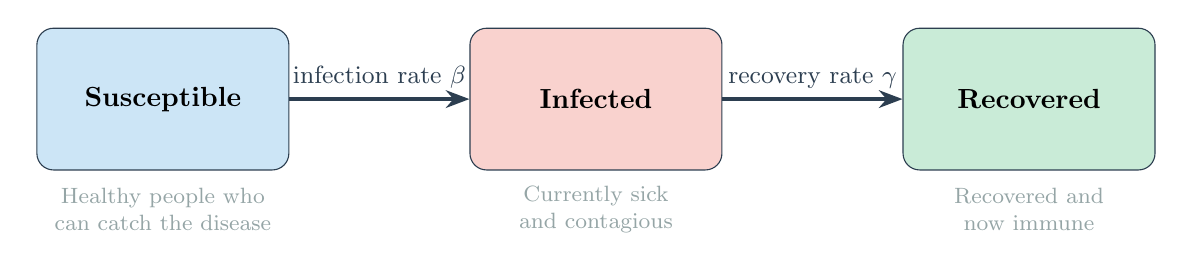
\begin{tikzpicture}[
    comp/.style={rectangle, rounded corners=6pt, draw=csprimary, fill=#1,
                 minimum width=32mm, minimum height=18mm, align=center, font=\bfseries},
    arrow/.style={-{Stealth[length=3mm]}, very thick, color=csprimary},
    sub/.style={font=\footnotesize, color=codegray, align=center, text width=32mm}
]
\node[comp=cstertiary!25] (S) at (0,0)   {\textbf{S}usceptible};
\node[comp=cssecondary!25](I) at (5.5,0) {\textbf{I}nfected};
\node[comp=csaccent!25]   (R) at (11,0)  {\textbf{R}ecovered};

\draw[arrow] (S) -- node[above, font=\small, color=csprimary] {infection rate $\beta$} (I);
\draw[arrow] (I) -- node[above, font=\small, color=csprimary] {recovery rate $\gamma$} (R);

\node[sub] at (0,-1.4)   {Healthy people who\\can catch the disease};
\node[sub] at (5.5,-1.4) {Currently sick\\and contagious};
\node[sub] at (11,-1.4)  {Recovered and\\now immune};
\end{tikzpicture}
\end{center}

Two parameters govern the model:
\begin{itemize}[itemsep=3pt]
    \item \textbf{$\beta$ (beta):} The infection rate---how quickly susceptible people become infected through contact with infected people.
    \item \textbf{$\gamma$ (gamma):} The recovery rate---how quickly infected people recover (and become immune).
\end{itemize}

Their ratio, $R_0 = \beta / \gamma$, is the \keyterm{basic reproduction number}: how many new infections one sick person causes in a fully susceptible population. If $R_0 > 1$, the disease spreads. If $R_0 < 1$, it fades out. You almost certainly heard this number discussed during the COVID-19 pandemic.

\begin{center}
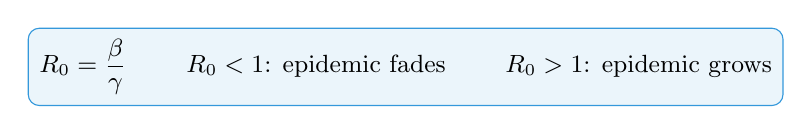
\begin{tikzpicture}
\node[font=\small, align=center, draw=cstertiary, fill=cstertiary!10,
      rounded corners=4pt, inner sep=4pt] at (0,0)
    {$R_0 = \dfrac{\beta}{\gamma}$ \quad\quad
     $R_0 < 1$: epidemic fades \quad\quad
     $R_0 > 1$: epidemic grows};
\end{tikzpicture}
\end{center}

\subsection{Discretizing the Math}

The SIR model is mathematically expressed as a set of \keyterm{differential equations} describing how the compartments change continuously over time. For our Java simulation, we convert these to \keyterm{difference equations}---small discrete time steps, each computing how much the population in each compartment changes. This technique is called \keyterm{Euler's method}, and it is the simplest approach to numerical simulation.

At each time step $\Delta t$:
\[
\Delta S = -\beta \cdot S \cdot I \cdot \Delta t
\qquad
\Delta I = \left(\beta \cdot S \cdot I - \gamma \cdot I\right) \cdot \Delta t
\qquad
\Delta R = \gamma \cdot I \cdot \Delta t
\]

In words: the number of newly infected people is proportional to both the number of susceptible people and the number of infectious people (they have to meet). The number recovering is proportional to the number currently infected.

\begin{javacode}[The SIR Epidemic Model in Java]
public class SIRModel {
    // Model parameters
    private double beta;    // infection rate (contacts per day * P(transmission))
    private double gamma;   // recovery rate (1 / average days sick)

    // Population compartments (as fractions: 0.0 to 1.0)
    private double S;       // fraction susceptible
    private double I;       // fraction infected
    private double R;       // fraction recovered

    public SIRModel(double beta, double gamma,
                    double initialInfected) {
        this.beta  = beta;
        this.gamma = gamma;
        this.I = initialInfected;
        this.S = 1.0 - initialInfected;
        this.R = 0.0;
    }

    // Advance the simulation by one time step (Euler's method)
    public void step(double dt) {
        double newlyInfected = beta * S * I * dt;
        double newlyRecovered = gamma * I * dt;

        S -= newlyInfected;
        I += newlyInfected - newlyRecovered;
        R += newlyRecovered;
    }

    // Run the full simulation and print a time series
    public void simulate(int days, double dt) {
        System.out.printf("%-6s  %-10s  %-10s  %-10s%n",
                          "Day", "Susceptible", "Infected", "Recovered");
        double t = 0;
        while (t <= days) {
            if (t % 10 < dt) {    // print every 10 days
                System.out.printf("%-6.0f  %-10.4f  %-10.4f  %-10.4f%n",
                                  t, S, I, R);
            }
            step(dt);
            t += dt;
        }
    }

    public double getR0() { return beta / gamma; }

    public static void main(String[] args) {
        // Flu-like parameters: R0 = 1.5 / 0.3 = 5
        SIRModel flu = new SIRModel(
            0.3,      // beta: 30% of contacts lead to infection per day
            0.1,      // gamma: recover in ~10 days on average
            0.001     // 0.1% of population initially infected
        );
        System.out.println("R0 = " + flu.getR0());
        flu.simulate(160, 0.1);
    }
}
\end{javacode}

\begin{tipbox}[Try It: Explore the Model]
After implementing this model, experiment with the parameters:
\begin{itemize}[itemsep=3pt]
    \item \textbf{Change $R_0$:} Set $\beta = 0.05$, $\gamma = 0.1$ (so $R_0 = 0.5$). Does the disease spread?
    \item \textbf{Simulate vaccination:} Start with \texttt{S = 0.4} (60\% vaccinated and immune). What happens to the peak infected population? This is \textit{herd immunity} in code.
    \item \textbf{Flatten the curve:} Reduce $\beta$ by half (representing social distancing). How does the peak change? Does the total eventually infected change?
    \item \textbf{Add a fourth compartment:} Modify the model to include an \textbf{E}xposed class (infected but not yet contagious): $S \to E \to I \to R$. This is the SEIR model used for COVID-19.
\end{itemize}
These questions---answered by running your simulation---are exactly what epidemiologists ask when advising governments during outbreaks.
\end{tipbox}

\subsection{The Ferguson Model and COVID-19}

\begin{historybox}[The Model That Shaped Lockdowns (2020)]
In March 2020, a team at Imperial College London led by Neil Ferguson published a model of COVID-19 spread. Its central finding: without intervention, the pandemic could kill 510,000 people in the UK and 2.2 million in the US.

Within days, the UK government reversed course from a ``herd immunity'' strategy to a lockdown. The US followed. The model---a sophisticated extension of ideas like the SIR model, running on millions of simulated individuals---directly influenced policy affecting billions of people.

The model was immediately scrutinized. Critics pointed to code quality issues, sensitivity to assumptions, and differences between the model's predictions and observed outcomes. Defenders noted that interventions \textit{changed} the outcome the model predicted---a lockdown that works looks like an over-prediction. The debate illustrated both the power and the responsibility of computational modeling: when a program shapes government policy, the quality of that code is a matter of public health.
\end{historybox}

%---------- MONTE CARLO ----------%
\section{Case Study: Monte Carlo Methods}

\subsection{Estimating with Randomness}

Some quantities are too complex to calculate directly but can be \textit{estimated} by random sampling. This family of techniques is called \keyterm{Monte Carlo methods}, named after the famous casino---because they rely on chance.

The most famous introduction to Monte Carlo is estimating $\pi$ by throwing imaginary darts.

\begin{center}
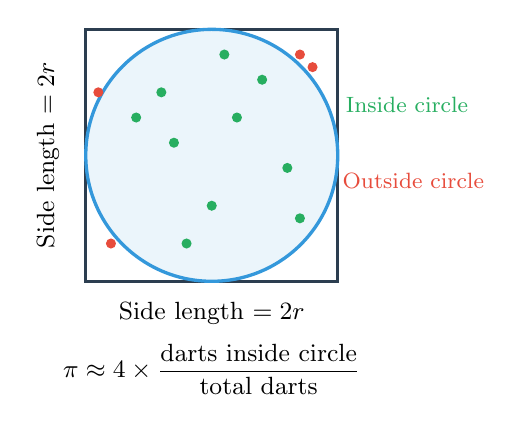
\begin{tikzpicture}[scale=1.6]
% Square
\draw[draw=csprimary, line width=1.2pt] (-1,-1) rectangle (1,1);
% Circle
\draw[draw=cstertiary, line width=1.2pt, fill=cstertiary!10] (0,0) circle (1);
% Axes labels
\node[font=\small] at (0,-1.25) {Side length $= 2r$};
\node[font=\small, rotate=90] at (-1.3,0) {Side length $= 2r$};
% Sample dots inside circle
\foreach \x/\y in {0.2/0.3, -0.4/0.5, 0.6/-0.1, -0.2/-0.7, 0.1/0.8,
                   -0.6/0.3, 0.4/0.6, -0.3/0.1, 0.7/-0.5, 0.0/-0.4} {
    \fill[csaccent] (\x,\y) circle (0.04);
}
% Sample dots outside circle
\foreach \x/\y in {0.8/0.7, -0.9/0.5, 0.7/0.8, -0.8/-0.7} {
    \fill[cssecondary] (\x,\y) circle (0.04);
}
% Annotations
\node[font=\footnotesize, color=csaccent] at (1.55,0.4) {Inside circle};
\node[font=\footnotesize, color=cssecondary] at (1.6,-0.2) {Outside circle};
% Formula
\node[font=\small, align=center] at (0,-1.7)
    {$\pi \approx 4 \times \dfrac{\text{darts inside circle}}{\text{total darts}}$};
\end{tikzpicture}
\end{center}

The logic: a circle of radius $r$ inscribed in a square of side $2r$ has area $\pi r^2$. The square has area $4r^2$. The fraction of the square covered by the circle is $\pi/4$. If we throw darts uniformly at random at the square, roughly $\pi/4$ of them will land inside the circle. Multiply the fraction by 4, and we get $\pi$.

\begin{javacode}[Monte Carlo Estimation of Pi]
import java.util.Random;

public class MonteCarloPi {

    public static double estimatePi(int numDarts) {
        Random rng = new Random();
        int insideCircle = 0;

        for (int i = 0; i < numDarts; i++) {
            // Throw a random dart at the unit square [-1,1] x [-1,1]
            double x = rng.nextDouble() * 2 - 1;   // random in [-1, 1]
            double y = rng.nextDouble() * 2 - 1;   // random in [-1, 1]

            // Is it inside the unit circle? x^2 + y^2 <= 1
            if (x * x + y * y <= 1.0) {
                insideCircle++;
            }
        }

        return 4.0 * insideCircle / numDarts;
    }

    public static void main(String[] args) {
        int[] dartCounts = {100, 1_000, 10_000, 100_000, 1_000_000};

        System.out.printf("%-12s  %-12s  %-12s%n",
                          "Darts", "Estimated Pi", "Error");
        for (int n : dartCounts) {
            double estimate = estimatePi(n);
            double error = Math.abs(estimate - Math.PI);
            System.out.printf("%-12d  %-12.6f  %-12.6f%n",
                              n, estimate, error);
        }
    }
}
\end{javacode}

Each time you run this program you get a slightly different answer---that's the nature of random sampling. The more darts you throw, the closer the estimate gets to the true value. The error shrinks proportionally to $1/\sqrt{n}$: to halve the error, you need four times as many samples.

\subsection{Where Monte Carlo Is Actually Used}

Estimating $\pi$ is a toy example, but the underlying technique is used throughout science and engineering:

\begin{itemize}[itemsep=4pt]
    \item \textbf{Nuclear physics:} The method was invented by physicists Stanislaw Ulam and John von Neumann in the 1940s to model neutron diffusion in nuclear reactors---too complex for analytical mathematics.

    \item \textbf{Climate science:} Running a climate model once gives one possible future. Running it thousands of times with slightly varied parameters generates a \textit{distribution} of futures, revealing which predictions are robust and which are sensitive to assumptions.

    \item \textbf{Financial risk:} Banks simulate millions of possible future market scenarios to estimate the probability of large losses (``Value at Risk'').

    \item \textbf{Drug discovery:} Pharmaceutical researchers simulate thousands of candidate molecules docking to protein targets, looking for promising drug candidates---a search space too large to explore experimentally.

    \item \textbf{Rendering in films:} The photorealistic lighting in animated films is computed using Monte Carlo ray tracing: tracing millions of random light paths to estimate how light would actually behave.
\end{itemize}

\begin{tipbox}[The Power of Sampling]
Monte Carlo methods reveal a profound idea: you often don't need to evaluate every possibility to understand a system. A well-chosen random sample can be nearly as informative as an exhaustive search, at a tiny fraction of the cost.

This same principle appears in statistics (surveys sample populations instead of asking everyone), in software testing (random test inputs find bugs that hand-crafted tests miss), and in machine learning (stochastic gradient descent trains models on random subsets of data, not the full dataset at once).

Whenever you face a problem where the full search space is too large to explore completely, ask: can I get a useful answer from a random sample?
\end{tipbox}

%---------- N-BODY AND PHYSICS SIM ----------%
\section{Case Study: Simulating the Solar System}

\subsection{The N-Body Problem}

Newton's law of gravity lets us calculate the force between any two objects. But what happens when there are three? Ten? A billion? The \keyterm{$N$-body problem}---predicting the motion of $N$ objects mutually attracting each other by gravity---has no general closed-form solution for $N \geq 3$. The only way to answer ``where will all these objects be in a million years?'' is to simulate it.

The approach is the same Euler time-stepping we used for the SIR model:

\begin{javacode}[A Simplified N-Body Simulation in Java]
public class Body {
    double x, y;       // position (meters)
    double vx, vy;     // velocity (meters/second)
    double mass;       // kilograms

    public Body(double x, double y, double vx, double vy, double mass) {
        this.x = x; this.y = y;
        this.vx = vx; this.vy = vy;
        this.mass = mass;
    }
}

public class NBodySimulation {
    private static final double G = 6.674e-11; // gravitational constant

    // Advance all bodies by one time step
    public static void step(Body[] bodies, double dt) {
        // For each body, compute the total gravitational force from all others
        double[] fx = new double[bodies.length];
        double[] fy = new double[bodies.length];

        for (int i = 0; i < bodies.length; i++) {
            for (int j = 0; j < bodies.length; j++) {
                if (i == j) continue;

                double dx = bodies[j].x - bodies[i].x;
                double dy = bodies[j].y - bodies[i].y;
                double dist = Math.sqrt(dx * dx + dy * dy);
                double force = G * bodies[i].mass * bodies[j].mass
                               / (dist * dist);

                // Decompose force into x and y components
                fx[i] += force * dx / dist;
                fy[i] += force * dy / dist;
            }
        }

        // Update velocities and positions using the computed forces
        for (int i = 0; i < bodies.length; i++) {
            bodies[i].vx += fx[i] / bodies[i].mass * dt;
            bodies[i].vy += fy[i] / bodies[i].mass * dt;
            bodies[i].x  += bodies[i].vx * dt;
            bodies[i].y  += bodies[i].vy * dt;
        }
    }
}
\end{javacode}

This same structure---compute forces between all pairs, update velocities, update positions---is used in molecular dynamics simulations that model protein folding, drug interactions, and materials science. The physics changes; the loop does not.

\subsection{What N-Body Simulations Have Revealed}

The simulation of gravitational systems has produced real scientific discoveries:

\begin{itemize}[itemsep=4pt]
    \item \textbf{Galaxy collisions:} Simulations in the 1970s showed that the Milky Way and Andromeda galaxies will collide in approximately 4.5 billion years---and revealed that such collisions, counterintuitively, rarely result in stellar collisions (galaxies are mostly empty space).

    \item \textbf{Planetary formation:} Simulations of dust and gas in a young solar system replicate the formation of rocky inner planets and gas giants, supporting the \textit{nebular hypothesis} with quantitative evidence.

    \item \textbf{The Moon's origin:} The leading theory---that the Moon formed when a Mars-sized body struck the early Earth---is supported primarily by simulations showing that such an impact would produce debris consistent with the Moon's composition.
\end{itemize}

%---------- WHEN MODELS GO WRONG ----------%
\section{When Models Go Wrong}

\subsection{Garbage In, Garbage Out}

A model is only as good as its inputs and assumptions. The acronym \keyterm{GIGO}---``garbage in, garbage out''---captures a fundamental truth: a correctly implemented model based on wrong assumptions produces wrong answers, often with false precision.

\begin{warningbox}[Famous Modeling Failures]
\textbf{Long-Term Capital Management (1998):} A hedge fund run by Nobel Prize-winning economists used sophisticated mathematical models to manage financial risk. Their models assumed that extreme market events were vanishingly rare---based on historical data that didn't include certain rare scenarios. When the Russian financial crisis created exactly such an event, the fund lost \$4.6 billion in weeks and required a Federal Reserve bailout to prevent broader financial contagion.

\textbf{The Tacoma Narrows Bridge (1940):} Engineers correctly modeled the static load the bridge could bear. They undermodeled the aerodynamic forces that could cause resonant oscillation. The bridge collapsed dramatically four months after opening, filmed in footage that became iconic in engineering education. The lesson: a model that ignores the wrong physics can be worse than no model at all.

\textbf{Early COVID-19 Models:} Multiple early models of COVID-19 spread made assumptions that turned out not to hold---about the fraction of cases that were asymptomatic, about how quickly immunity waned, about how much behavior would change in response to interventions. Some predictions were dramatically wrong. This doesn't mean the models were useless---they shaped policy that saved lives---but it illustrates that model uncertainty should always be explicitly communicated alongside predictions.
\end{warningbox}

\subsection{Validation and Sensitivity Analysis}

Two practices help modelers avoid overconfidence in their results:

\textbf{Validation} means testing the model against data it wasn't fitted to. If a climate model trained on data from 1900--1970 correctly predicts temperatures from 1970--2000, that's evidence it captures real physics. If it fails, the model needs revision.

\textbf{Sensitivity analysis} means systematically varying the model's parameters and assumptions to see how much the outputs change. If the conclusion changes dramatically when one assumption is tweaked slightly, that's a warning: the conclusion is fragile and should be held less confidently. If the conclusion is robust across a wide range of assumptions, it can be trusted more.

\begin{javacode}[Simple Sensitivity Analysis with the SIR Model]
public static void sensitivityAnalysis() {
    // How does peak infection depend on the infection rate beta?
    double gamma = 0.1;
    double[] betaValues = {0.15, 0.20, 0.25, 0.30, 0.35, 0.40};

    System.out.printf("%-8s  %-6s  %-18s  %-16s%n",
                      "Beta", "R0", "Peak Infected (%)", "Day of Peak");

    for (double beta : betaValues) {
        SIRModel model = new SIRModel(beta, gamma, 0.001);
        double peakI = 0;
        int peakDay = 0;
        for (int day = 0; day <= 200; day++) {
            for (int step = 0; step < 10; step++) model.step(0.1);
            if (model.getI() > peakI) {
                peakI = model.getI();
                peakDay = day;
            }
        }
        System.out.printf("%-8.2f  %-6.1f  %-18.1f  %-16d%n",
                          beta, beta / gamma, peakI * 100, peakDay);
    }
}
\end{javacode}

Running this reveals how sensitive epidemic severity is to the infection rate---exactly the question public health officials ask when evaluating interventions like masking or school closures.

\subsection{The Ethics of Modeling}

When models influence major decisions---pandemic policy, nuclear reactor design, financial regulation, climate legislation---questions of responsibility arise.

\begin{debatebox}[Who Is Responsible When a Model Is Wrong?]
\textbf{Transparency:} Should scientific models used in policy be publicly available? Open-source models can be scrutinized and improved by the community; proprietary models cannot. There is growing pressure in science for \textbf{open science}: publishing not just results but data and code.

\textbf{Uncertainty communication:} Models almost always produce a range of outcomes, not a single number. When policymakers receive a single number---``510,000 deaths without intervention''---they often treat it as a precise prediction rather than the center of a wide distribution. Modelers have a responsibility to communicate uncertainty clearly, even when policymakers prefer simple answers.

\textbf{Model advocacy:} Researchers sometimes have views on what policies should follow from their models. When does a scientist appropriately inform a policy discussion, and when do they cross into advocacy? This line is genuinely contested.

\textbf{Access and inequality:} Nations with computational infrastructure can develop sophisticated models; poorer nations often cannot. During COVID-19, wealthy countries with well-developed epidemiological modeling capacity made different---and generally better-informed---decisions than those without.
\end{debatebox}

%---------- THE CAREER LANDSCAPE ----------%
\section{Computational Science as a Career}

\subsection{A New Kind of Scientist}

The rise of computational modeling has created a new kind of scientist: the \keyterm{computational scientist} or \keyterm{research software engineer}. These roles sit at the intersection of domain expertise (biology, physics, climate science, economics) and software engineering.

\begin{conceptbox}[What Computational Scientists Do]
\begin{itemize}[itemsep=3pt]
    \item \textbf{Climate scientists} write and run global circulation models to project future temperature, precipitation, and sea level.
    \item \textbf{Bioinformaticians} analyze genomic data, building pipelines that process terabytes of sequencing output.
    \item \textbf{Computational chemists} simulate molecular interactions to understand reaction mechanisms and discover new materials.
    \item \textbf{Epidemiological modelers} build disease models to inform vaccine strategies and outbreak responses.
    \item \textbf{Astrophysicists} simulate galaxy formation, black hole mergers, and the large-scale structure of the universe.
    \item \textbf{Quantitative social scientists} use agent-based models to study economic behavior, social network dynamics, and policy effects.
\end{itemize}
In most of these fields, the ability to write good code is now as fundamental as the ability to design an experiment or derive an equation.
\end{conceptbox}

\subsection{Tools of the Trade}

Most computational science today is done in \textbf{Python}---specifically its scientific ecosystem: \texttt{NumPy} for numerical arrays, \texttt{SciPy} for scientific algorithms, \texttt{matplotlib} for plotting, and \texttt{pandas} for data analysis. \textbf{R} is widely used in statistics and biology. \textbf{Julia} is a newer language designed specifically for high-performance scientific computing. \textbf{MATLAB} remains common in engineering.

Java is less common in front-line computational science but appears in large simulation frameworks (the \textbf{NetLogo} agent-based modeling platform compiles to the JVM; many geospatial and bioinformatics tools are Java-based). More importantly, the concepts you learn in Java---loops, objects, interfaces, data structures---transfer directly to any computational science language.

\begin{tipbox}[From Java to Scientific Computing]
If computational science interests you, your Java foundation transfers well:
\begin{itemize}[itemsep=3pt]
    \item \textbf{Python} is syntactically simpler than Java; most Java programmers can read Python code immediately. The \texttt{NumPy} library makes array operations that would require nested loops in Java into single expressions.
    \item \textbf{Jupyter notebooks} let you write code and see results in the same document---ideal for exploratory science. They run Python (and other languages) in a web browser.
    \item \textbf{NetLogo} is a free agent-based modeling environment with a gentle learning curve, specifically designed for non-programmers building simulations.
    \item The SIR model and Monte Carlo examples in this case study are straightforward to port to Python---try it as an exercise.
\end{itemize}
\end{tipbox}

%---------- DISCUSSION QUESTIONS ----------%
\section*{Discussion Questions}

\begin{questionbox}
\begin{enumerate}[leftmargin=*, label=\textcolor{cswarm}{\textbf{\arabic*.}}]
    \item \textbf{``All Models Are Wrong'':} George Box's aphorism says all models are wrong, but some are useful. What makes a wrong model useful? Can you think of a model (in science, economics, or everyday life) that is clearly a simplification of reality but still provides genuine insight?

    \item \textbf{Validation and Trust:} The Ferguson COVID-19 model was criticized after the pandemic unfolded differently from some predictions. Does that mean the model was bad? What would you need to know to fairly evaluate whether a model was good or bad? How should society decide which models to trust?

    \item \textbf{Lorenz's Discovery:} Edward Lorenz discovered chaos theory by accident, noticing that a tiny change in input produced a wildly different simulation. What does this imply about long-range weather forecasting? About predicting other complex systems---economies, ecosystems, social trends? Are there limits to what computation can predict?

    \item \textbf{Sensitivity Analysis:} Run the sensitivity analysis from this case study (or trace through it by hand). How does the day of peak infection change as $R_0$ increases from 1.5 to 4? What does this tell you about the importance of early intervention in an epidemic?

    \item \textbf{Open Science:} Should scientific models used to influence public policy always be publicly available---code and all? What are the arguments for and against? Who should decide?
\end{enumerate}
\end{questionbox}

%---------- GLOSSARY ----------%
\section*{Key Terms}

\begin{glossarybox}
\begin{description}[leftmargin=!, labelwidth=3.8cm, font=\bfseries\color{cssecondary}]
    \item[Basic Reproduction Number ($R_0$)] The average number of new infections one infected individual causes in a fully susceptible population; if $R_0 > 1$ the disease spreads.

    \item[Butterfly Effect] The phenomenon whereby tiny differences in initial conditions lead to vastly different outcomes in chaotic systems; discovered computationally by Edward Lorenz in 1961.

    \item[Chaos Theory] The study of systems that are sensitively dependent on initial conditions, making long-range prediction fundamentally impossible despite being deterministic.

    \item[Compartmental Model] A model that divides a population into groups (compartments) and tracks the flow of individuals between them; the SIR model is a classic example.

    \item[Computational Model] A program that encodes the rules governing a system and simulates its behavior over time, used when systems are too complex for analytical mathematics.

    \item[Delta Time / Time Step ($\Delta t$)] The small increment of simulated time used in a numerical simulation; smaller steps give more accurate results but require more computation.

    \item[Differential Equation] A mathematical equation relating a quantity to its rate of change; the continuous-time basis for many scientific models.

    \item[Euler's Method] A simple technique for numerically integrating differential equations by approximating them as small finite steps.

    \item[GIGO] ``Garbage In, Garbage Out'': a model based on incorrect inputs or assumptions will produce incorrect outputs regardless of how correctly it is implemented.

    \item[Monte Carlo Method] A computational technique that uses random sampling to estimate quantities too complex to calculate directly.

    \item[$N$-Body Problem] The problem of predicting the motion of $N$ mutually gravitating objects; has no general closed-form solution for $N \geq 3$ and must be simulated numerically.

    \item[Sensitivity Analysis] Systematically varying a model's parameters to determine how much the outputs depend on each assumption; fragile conclusions change dramatically with small parameter changes.

    \item[SIR Model] A compartmental epidemic model dividing a population into Susceptible, Infected, and Recovered individuals; foundational in epidemiology.

    \item[Validation] Testing a model's predictions against data it was not used to build; the primary way to establish whether a model captures real phenomena.
\end{description}
\end{glossarybox}

\vspace{5mm}

%---------- FOOTER ----------%
\begin{center}
\textcolor{csprimary}{\rule{0.6\textwidth}{0.5pt}}\\[3mm]
{\small\textcolor{gray}{This case study is part of the Open Educational Resources for \cscourse.\\
Licensed under Creative Commons Attribution 4.0 (CC BY 4.0).}}
\end{center}

\end{document}
